\chapter{Background and Related Work}
\label{sec:background}

Computational experiments and simulation workflows now produce large volumes of scientific data \cite{boulakia2017workflows,wilkinson2025fairworkflows,villamar2025metadata}. In principle, this data can be modeled and validated directly with \gls{rdf}-based standards \cite{rdf_concepts2014,shacl_standard}. In day-to-day practice, however, many researchers still work with spreadsheets or with machine-readable formats such as \gls{xml} and \gls{json} rather than native \gls{rdf} graphs \cite{metaconfigurator2024,neubauer2026data}.

The Semantic Web promises better interoperability, explicit semantics, and cross-dataset integration \cite{berners2001semantic,janowicz2015geospatial,hogan2021knowledgegraphs}, but adopting it remains challenging. Typical hurdles include ontology engineering effort, identifier and vocabulary design, and mapping complexity \cite{janowicz2015geospatial,hogan2021knowledgegraphs}. To build a practical path through this gap, this chapter starts with \gls{json} and JSON Schema, then introduces core Semantic Web concepts, and finally positions MetaConfigurator as a schema-driven environment for data modeling and editing.

The chapter also reviews related tools for ontology engineering, data transformation, and semantic data management. Many of these tools are strong in their own scope but are commonly used in isolation. As a result, users often have to switch environments to move from structured \gls{json} data to semantically enriched \gls{rdf}. This thesis addresses that workflow gap by extending MetaConfigurator with semantic transformation, \gls{rdf} authoring, querying, and visualization in a single user-facing workflow.

\section{JSON and JSON Schema}

This section introduces the data foundations that many scientific workflows already rely on. It first discusses \gls{json} as a lightweight format for structured experimental data, then shows how JSON Schema adds machine-readable structural constraints. Together, they provide a pragmatic baseline for data quality before semantic enrichment and transformation into \gls{rdf}-based representations.

\subsection{JSON as a Data Representation Format}
\label{sec:background:json}

\gls{json} is a lightweight data-interchange format widely used for representing structured data in web services, scientific workflows, and configuration systems. \gls{json} encodes data as attribute-value pairs and ordered lists, making it both human-readable and machine-parseable. Due to its simplicity and broad ecosystem support, \gls{json} has become a de facto standard for structured data exchange across many domains \cite{json_standard}.

\begin{lstlisting}[float=htbp,style=json,caption={Example JSON representation of simulation input parameters and results}, label={lst:background_json_example}]
{
  "parameters": [
    {
      "name": "element_size",
      "value": 0.025,
      "unit": "M"
    }
  ],
  "metrics": [
    {
      "name": "max_von_mises_stress",
      "value": 299791507.5586333,
      "unit": "MegaPA"
    }
  ]
}
\end{lstlisting}

The running example is derived from the benchmark concept presented by Unger et al. for validation and verification of simulation models for concrete structures \cite{Unger2026Platform}. The benchmark context is a real finite-element simulation setting in which comparable test cases are executed across tools and mesh resolutions to evaluate reproducibility and implementation consistency. In such a setup, each run must be documented in a machine-readable form so that results can be compared, queried, and reproduced.

Listing~\ref{lst:background_json_example} shows one such run record as two arrays: \texttt{parameters} for model inputs and \texttt{metrics} for computed outputs. Each entry follows the structure \texttt{name}, \texttt{value}, and \texttt{unit}. In this example, \texttt{element\_size} is the characteristic mesh length for \(h\)-refinement (here \(0.025\,\mathrm{m}\), where smaller values mean finer meshes), and \texttt{max\_von\_mises\_stress} is the resulting maximum von Mises stress of the simulated specimen (approximately \(299.8\,\mathrm{MPa}\)) \cite{Unger2026Platform}. 

While \gls{json} provides a convenient serialization format, it does not inherently enforce structural constraints. Therefore, additional mechanisms are required to validate that \gls{json} documents conform to an expected structure.

\subsection{JSON Schema for Data Validation}
\label{sec:background:json_jsonschema}

JSON Schema offers a standard way to describe the expected structure and constraints of \gls{json} documents. A schema defines properties, data types, required attributes, and validation rules for JSON instances, enabling automated quality checks. The JSON Schema specification formalizes this vocabulary for describing \gls{json} documents and their validation behavior \cite{wright2020jsonschema}. 

Listing~\ref{lst:background_json_schema} presents a JSON Schema corresponding to the example \gls{json} document in Listing~\ref{lst:background_json_example}. The schema mirrors the structure of the instance and ensures that the document contains the expected \texttt{parameters} and \texttt{metrics} arrays. Each entry in these arrays follows a common structure with the fields \texttt{name}, \texttt{value}, and \texttt{unit}, enforcing that every variable has a textual identifier, a numeric value, and an associated unit.

The schema in Listing~\ref{lst:background_json_schema} checks that simulation data has the expected format before it is processed further. It requires every parameter and metric to include a \texttt{name}, a numeric \texttt{value}, and a \texttt{unit}, and it blocks unexpected extra fields (\texttt{additionalProperties: false}). This avoids common exchange problems such as missing units, wrong field names, or incorrect data types. At the same time, JSON Schema focuses on structural validity only: it does not encode the domain meaning of terms such as \texttt{element\_size} or \texttt{max\_von\_mises\_stress}, nor does it provide semantic interoperability with \glspl{kg}. To address this limitation, semantic mapping techniques are required.

\begin{lstlisting}[float=htbp,style=json, caption={JSON Schema validating the simulation result for JSON document in Listing~\ref{lst:background_json_example}}, label={lst:background_json_schema}]
{
  "$schema": "https://json-schema.org/draft/2020-12/schema",
  "title": "Simulation Parameters and Results Dataset",
  "description": "Schema describing input parameters and resulting performance metrics of a simulation run.",
  "type": "object",
  "properties": {
    "parameters": {
      "title": "Simulation Input Parameters",
      "description": "List of input variables.",
      "type": "array",
      "items": {
        "$ref": "#/$defs/variable"
      }
    },
    "metrics": {
      "title": "Simulation Metrics",
      "description": "List of measured or computed results produced by the simulation.",
      "type": "array",
      "items": {
        "$ref": "#/$defs/variable"
      }
    }
  },
  "required": [
    "parameters",
    "metrics"
  ],
  "additionalProperties": false,
  "$defs": {
    "variable": {
      "title": "Quantitative Variable",
      "description": "Represents a numeric quantity with a name and unit, used for both parameters and metrics.",
      "type": "object",
      "properties": {
        "name": {
          "title": "Variable Name",
          "type": "string",
          "description": "Identifier of the parameter or metric."
        },
        "value": {
          "title": "Numeric Value",
          "type": "number",
          "description": "Measured or assigned numeric value."
        },
        "unit": {
          "title": "Measurement Unit",
          "type": "string",
          "description": "Unit symbol following a standard QUDT instance."
        }
      },
      "required": [
        "name",
        "value",
        "unit"
      ],
      "additionalProperties": false
    }
  }
}
\end{lstlisting}

\section{Semantic Web}

The Semantic Web extends the World Wide Web by enabling data to be represented in a machine-readable, semantically rich form. This allows heterogeneous data to be interlinked, interpreted consistently, and queried across systems \cite{berners2001semantic}.

\subsection{Ontology: Modeling Knowledge Domains}
\label{sec:background:ontology}

Ontologies provide a formal specification of concepts and relationships within a domain of knowledge.
One of the most widely cited and influential definitions is provided by Gruber~\cite{gruber1993ontology}:
\begin{quote}
``An ontology is an \underline{explicit} \underline{specification} of a \underline{shared conceptualization}.'' 
\end{quote}

In the context of scientific experiments, ontologies can define experiment parameters, measurement units, procedures, and results. For example, an ontology might define a class 
\href{https://schema.org/PropertyValue}{\texttt{PropertyValue}} 
representing any measured property, a class 
\href{https://nfdi4ing.pages.rwth-aachen.de/metadata4ing/metadata4ing/\#Method}{\texttt{Method}} 
representing experimental procedures, and relationships such as 
\href{https://nfdi4ing.pages.rwth-aachen.de/metadata4ing/metadata4ing/\#hasParameter}{\texttt{hasParameter}} 
and 
\href{https://nfdi4ing.pages.rwth-aachen.de/metadata4ing/metadata4ing/\#investigates}{\texttt{investigates}} 
to link methods to parameters and observed metrics.

Ontologies serve as the backbone for semantic data integration and reasoning. They allow data from heterogeneous sources to be interpreted consistently, facilitate interoperability, and enable advanced queries across datasets using formal reasoning engines.

\subsection{RDF: Resource Description Framework}
\label{sec:background:rdf}

\gls{rdf} is the core data model of the Semantic Web. It represents information as triples of \textit{subject}, \textit{predicate}, and \textit{object}, which together form a graph structure \cite{rdf_concepts2014}. This model provides a common, tool-independent way to express entities and relationships across datasets.

Formally, a \gls{rdf} triple is a 3-tuple \cite{rdf_concepts2014}:
\[
(s, p, o) \in (U \cup B) \times U \times (U \cup B \cup L)
\]
where:
\begin{itemize}
    \item \(U\) is the set of all \glspl{iri},
    \item \(B\) is the set of blank nodes (anonymous resources),
    \item \(L\) is the set of \gls{rdf} literals (e.g., strings, numbers, dates),
    \item \(s \in U \cup B\) is the subject,
    \item \(p \in U\) is the predicate (also called property),
    \item \(o \in U \cup B \cup L\) is the object.
\end{itemize}
A \gls{rdf} graph \(G\) is then defined as a finite set of such triples:
\[
G = \{(s_i, p_i, o_i) \mid i = 1, \dots, n\}, \quad s_i \in U \cup B, \; p_i \in U, \; o_i \in U \cup B \cup L
\]

\begin{lstlisting}[float=htbp,style=xml, caption={RDF/XML representation of parameter \texttt{element\_size} from Listing~\ref{lst:background_json_example}}, label={lst:background_rdf_xml_example}]
<rdf:RDF
 xmlns:rdf="http://www.w3.org/1999/02/22-rdf-syntax-ns#"
 xmlns:schema="https://schema.org/">
    <schema:PropertyValue rdf:about="https://www.example.org/variable_element_size">
        <schema:name>element_size</schema:name>
        <schema:unitCode rdf:resource="http://qudt.org/vocab/unit/M"/>
        <schema:value rdf:datatype="http://www.w3.org/2001/XMLSchema#double">2.5E-2</schema:value>
    </schema:PropertyValue>
</rdf:RDF>
\end{lstlisting}

\newpage

The RDF model in Listing~\ref{lst:background_rdf_xml_example} adds an extra layer of meaning to the same data in Listing~\ref{lst:background_json_example}. RDF/XML models the data as explicit graph statements instead of nested key-value objects, as depicted in Figures~\ref{fig:rdf:diagram_1} and \ref{fig:rdf:triples}\footnote{Visualization and Table view were generated with ISSemantic: \url{https://issemantic.net/}}. In JSON, fields such as \texttt{name}, \texttt{unit}, and \texttt{value} are interpreted mainly by application logic, whereas in RDF the subject (\texttt{variable\_element\_size}) is connected through well-defined predicates (\texttt{schema:name}, \texttt{schema:unitCode}, \texttt{schema:value}) to typed objects, including links to specific ontologies such as \gls{qudt}. This makes the representation less format-specific and more interoperable, because the meaning is encoded directly in standard \gls{iri} and data types rather than implied by local JSON structure.

\begin{figure}[htbp]
  \centering
  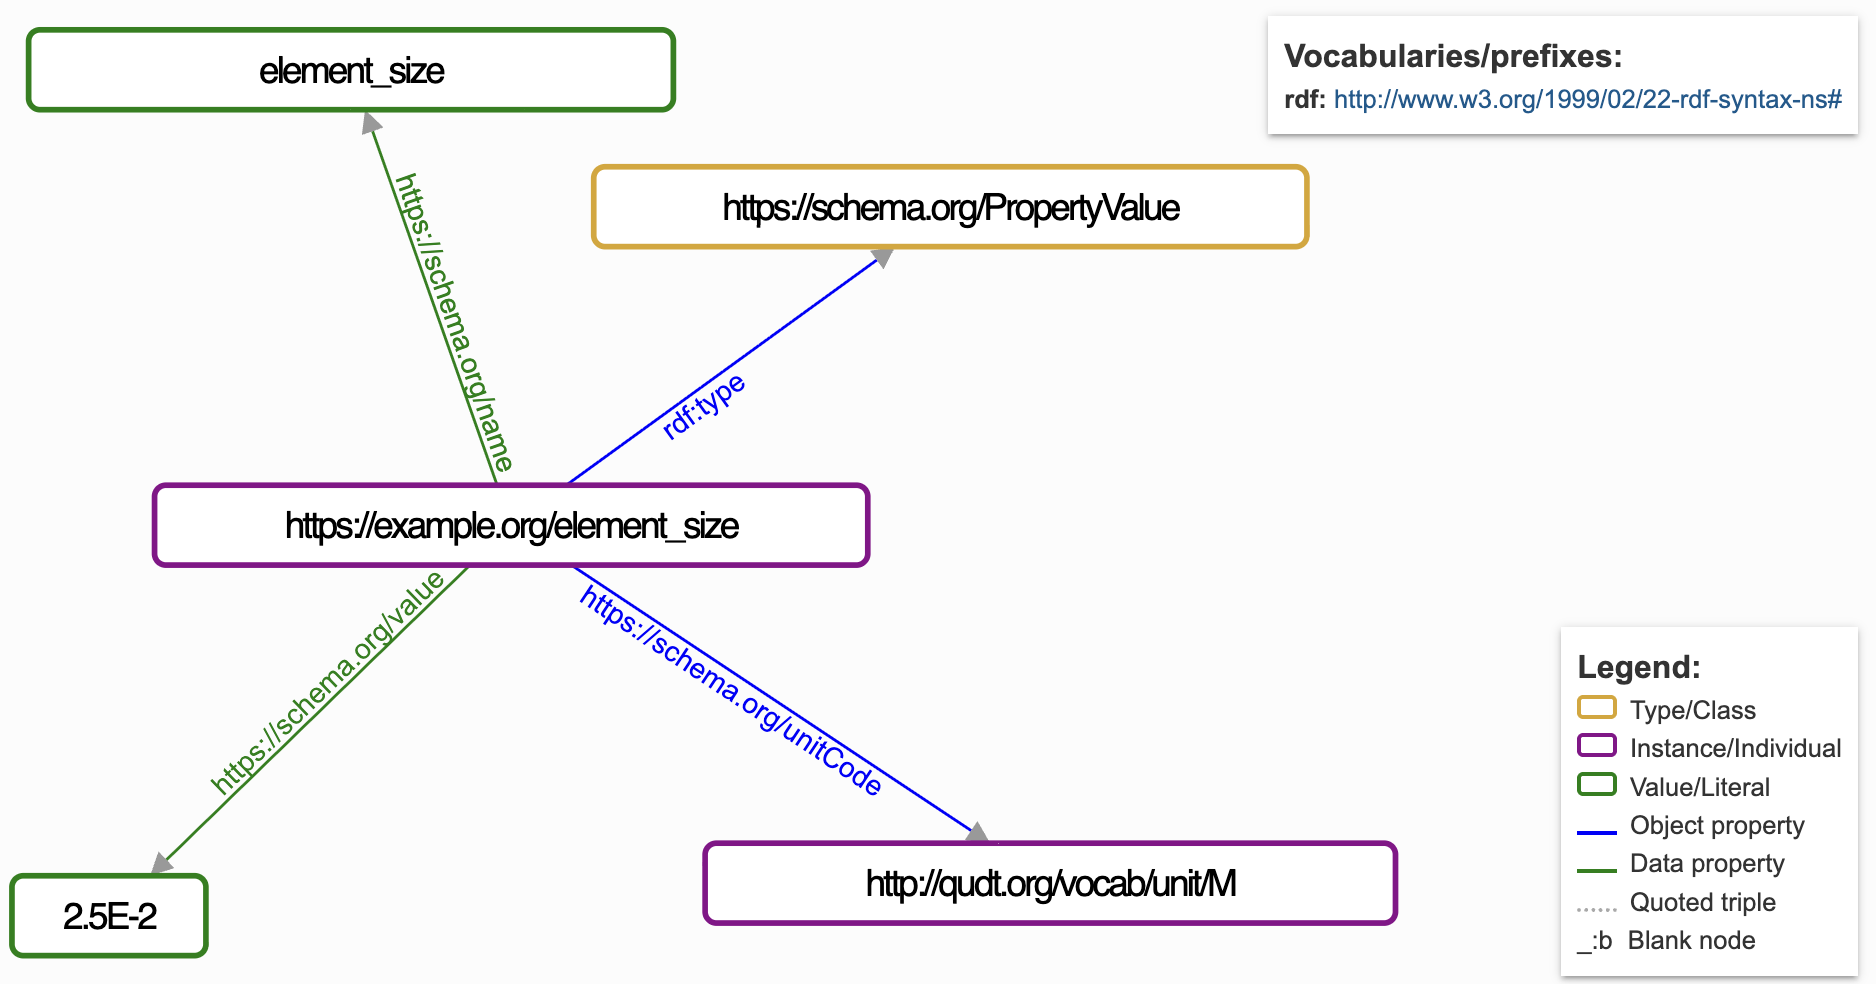
\includegraphics[width=.99\linewidth]{../figures/RDF-Diag-1.png}
  \caption{Graph view of the RDF representation in Listing~\ref{lst:background_rdf_xml_example}}
  \label{fig:rdf:diagram_1}
\end{figure}

\begin{figure}[htbp]
  \centering
  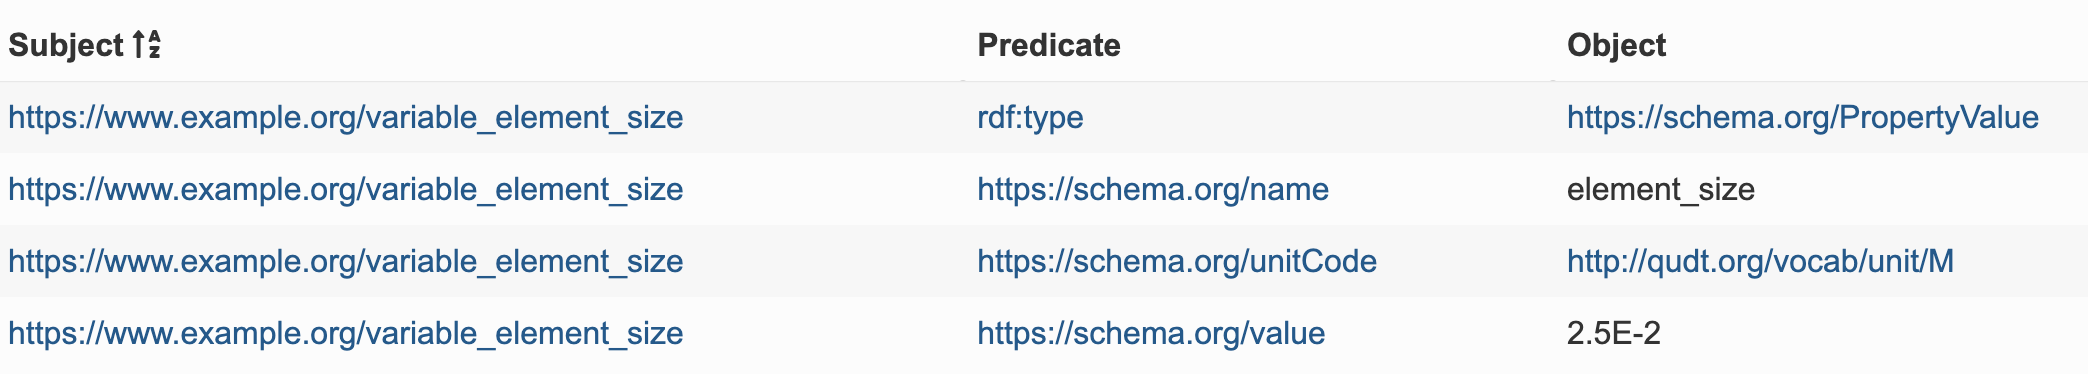
\includegraphics[width=.99\linewidth]{../figures/RDF-Triples.png}
  \caption{Table view of the RDF representation in Listing~\ref{lst:background_rdf_xml_example}}
  \label{fig:rdf:triples}
\end{figure}

\newpage

\subsection{JSON-LD as Serialization of RDF}
\label{sec:background:jsonld}

\gls{jsonld} is another serialization format for \gls{rdf} graphs, but expressed in \gls{json} syntax \cite{jsonld2014}. While RDF/XML (Listing~\ref{lst:background_rdf_xml_example}) uses XML tags, \gls{jsonld} represents the same graph concepts in a \gls{json} structure that is often easier to integrate into existing data pipelines and web-based tools.

A typical \gls{jsonld} document has two key structural components:

\begin{itemize}
    \item \texttt{@context:} This section defines the mapping between \gls{json} keys and ontology \glspl{iri} or vocabularies. It provides semantic meaning to each field.
    \item \texttt{@graph:} This array contains the actual data entities, each represented as a node with \texttt{@id}, \texttt{@type}, and associated properties. Relationships between entities are expressed using references to other \texttt{@id} values, forming a connected graph structure.
\end{itemize}

Listing~\ref{lst:background_jsonld_example} shows a complete \gls{jsonld} representation corresponding to the example in Listing~\ref{lst:background_json_example}. The \texttt{@context} defines prefixes such as \href{https://schema.org/}{\texttt{schema}} and \href{https://qudt.org/vocab/unit}{\texttt{unit}}, while the \texttt{@graph} contains nodes representing the simulation run, the \texttt{element\_size} parameter, and the stress metric.

\begin{lstlisting}[float=htbp,style=json, caption={JSON-LD representation of the simulation result presented in Listing~\ref{lst:background_json_example}}, label={lst:background_jsonld_example}]
{
  "@context": {
    "m4i": "http://w3id.org/nfdi4ing/metadata4ing#",
    "schema": "https://schema.org/",
    "unit": "http://qudt.org/vocab/unit/",
    "local": "https://www.example.org/"
  },
  "@graph": [
    {
      "@id": "local:run_fenics_simulation",
      "@type": "m4i:Method",
      "m4i:hasParameter": {
        "@id": "local:variable_element_size"
      },
      "m4i:investigates": {
        "@id": "local:variable_max_von_mises_stress"
      }
    },
    {
      "@id": "local:variable_element_size",
      "@type": "schema:PropertyValue",
      "schema:name": "element_size",
      "schema:unitCode": {
        "@id": "unit:M"
      },
      "schema:value": {
        "@type": "http://www.w3.org/2001/XMLSchema#double",
        "@value": "2.5E-2"
      }
    },
    {
      "@id": "local:variable_max_von_mises_stress",
      "@type": "schema:PropertyValue",
      "schema:name": "max_von_mises_stress",
      "schema:unitCode": {
        "@id": "unit:MegaPA"
      },
      "schema:value": {
        "@type": "http://www.w3.org/2001/XMLSchema#double",
        "@value": "2.997915075586333E8"
      }
    }
  ]
}
\end{lstlisting}

By modeling the experimental data from Listing~\ref{lst:background_json_example} in \gls{jsonld} and explicitly defining its semantics, the data becomes linked to the Semantic Web and can be integrated into a \gls{kg}. In this representation, \texttt{element\_size} is modeled as a \href{https://schema.org/PropertyValue}{\texttt{schema:PropertyValue}} resource with a typed numeric value and an explicit unit \gls{iri}, just as in RDF/XML. Compared with Listing~\ref{lst:background_rdf_xml_example}, the semantics are equivalent, but the syntax remains JSON-based.

\subsection{SHACL: Shapes Constraint Language}
\label{sec:background:shacl}

The \gls{shacl} is a \gls{w3c} standard for validating \gls{rdf} graphs against a set of structural and semantic constraints \cite{shacl_standard}. \gls{shacl} performs validation based on explicitly defined ``shapes'' \,that describe the expected properties, data types, and cardinality of \gls{rdf} nodes. 

While these shapes can be designed to reflect or align with domain ontologies, \gls{shacl} validation itself is independent of ontology languages such as \gls{owl}, which are primarily used for logical reasoning rather than constraint checking.

For example, consider the simulation parameter \texttt{element\_size} in the \gls{jsonld} example (Listing~\ref{lst:background_jsonld_example}). Using \gls{shacl}, we can define a shape that enforces that every \href{https://schema.org/PropertyValue}{\texttt{schema:PropertyValue}} representing an experiment parameter must have a numeric \href{https://schema.org/value}{\texttt{schema:value}} and a \href{https://schema.org/unitCode}{\texttt{schema:unitCode}} pointing to a valid unit from the \gls{qudt} ontology. By applying this shape, \gls{rdf} data can be automatically checked for compliance with the expected structure and semantics, preventing errors or inconsistencies before integration into a \gls{kg}.

\begin{lstlisting}[float=htbp,style=turtle, caption={SHACL shape for validating simulation parameters}, label={lst:background_shacl_example}]
@prefix sh: <http://www.w3.org/ns/shacl#> .
@prefix schema: <https://schema.org/> .
@prefix rdfs: <http://www.w3.org/2000/01/rdf-schema#> .
@prefix unit: <http://qudt.org/vocab/unit/> .
@prefix xsd: <http://www.w3.org/2001/XMLSchema#> .
@prefix local: <https://www.example.org/> .

local:PropertyValueShape
    a sh:NodeShape ;
    sh:targetClass schema:PropertyValue ;

    # The variable name label
    sh:property [
        sh:path rdfs:label ;
        sh:datatype xsd:string ;
        sh:minCount 1 ;
        sh:maxCount 1 ;
    ] ;

    # The numeric value of the parameter or metric
    sh:property [
        sh:path schema:value ;
        sh:datatype xsd:double ;
        sh:minCount 1 ;
        sh:maxCount 1 ;
    ] ;

    # The unit, as a named QUDT IRI
    sh:property [
        sh:path schema:unitCode ;
        sh:nodeKind sh:IRI ;
        sh:class qudt:Unit ;
        sh:minCount 1 ;
        sh:maxCount 1 ;
    ] .
\end{lstlisting}

\subsection{SPARQL: Querying Semantic Data}
\label{sec:background:sparql}

\gls{sparql} is the standard query language for \gls{rdf} datasets \cite{sparql_standard}, supporting retrieval, filtering, and aggregation of data stored in \glspl{kg}. Queries are expressed using triple patterns, similar to \gls{rdf} statements.

Listing~\ref{lst:background_sparql_example} presents an SPARQL example using the \gls{jsonld} simulation data, where all experiment parameters and metrics are retrieved together with their corresponding values and units.

\begin{lstlisting}[float=htbp,style=sparql, caption={SPARQL query retrieving parameter values and units}, label={lst:background_sparql_example}]
PREFIX schema: <https://schema.org/>
PREFIX rdfs: <http://www.w3.org/2000/01/rdf-schema#>
PREFIX unit: <http://qudt.org/vocab/unit/>
PREFIX local: <https://www.example.org/>

SELECT ?parameter ?value ?unit
WHERE {
    ?param a schema:PropertyValue ;
           rdfs:label ?parameter ;
           schema:value ?value ;
           schema:unitCode ?unit .
}
\end{lstlisting}

This query retrieves the parameters \texttt{element\_size} and \texttt{max\_von\_mises\_stress} together with their corresponding numeric values and associated \gls{qudt} units 
(\href{https://qudt.org/vocab/unit/M}{\texttt{unit:M}} and \href{https://qudt.org/vocab/unit/MegaPA}{\texttt{unit:MegaPA}}). The result reflects the structure of the JSON-LD representation, in which both parameters and metrics are modeled as \href{https://schema.org/PropertyValue}{\texttt{schema:PropertyValue}} resources.

This example illustrates how semantic annotations enable structured and consistent access to data. 
\gls{sparql} further provides mechanisms for querying \gls{rdf} graphs, including filtering and combining data from multiple sources, which supports the analysis of semantically enriched simulation data.

\newpage

\subsection{OWL: Modeling Rich Semantics and Logical Rules}
\label{sec:background:owl}

While \gls{rdf} provides the graph structure and \gls{sparql} enables querying, \gls{owl} adds a formal layer for expressing richer domain knowledge \cite{owl2_overview,owl2_primer}. With \gls{owl}, one can define class hierarchies, equivalence and disjointness of classes, and logical constraints on properties (e.g., transitive, symmetric, or cardinality-based restrictions). This allows data to be interpreted not only as stored triples, but also through the rules encoded in the ontology. As discussed in Section~\ref{sec:background:shacl}, \gls{shacl} complements this by providing a validation layer for structural and integrity constraints over \gls{rdf} graphs. Unlike \gls{owl}, which focuses on logical inference, \gls{shacl} is primarily used to validate whether data conforms to expected shapes, such as required properties, value types, or cardinality restrictions. Together, these technologies support a comprehensive workflow in which \gls{rdf} represents data, \gls{owl} enriches its semantics, \gls{sparql} enables flexible querying, and \gls{shacl} ensures data quality and conformance. 

Listing \ref{lst:background_owl_example} shows an example of an \gls{owl} property definition for \texttt{:hasParameter} in the Metadata4Ing ontology \cite{metadata4ing_ontology}. This property is defined as an object property with a domain that is a union of the classes \texttt{:Method} and \texttt{:Tool}, and a range that points to the class \texttt{Variable} from the PIMS-II\footnote{The PIMS-II (Process and Instrument Metadata Schema II) ontology is used to model variables and metadata associated with scientific and engineering processes, particularly in simulation and experimental workflows.} ontology. The definition also includes a human-readable comment and label.

\begin{lstlisting}[float=htbp,style=turtle, caption={Definition for \texttt{:hasParameter} property in Metadata4Ing ontology\cite{metadata4ing_ontology}}, label={lst:background_owl_example}]
:hasParameter rdf:type owl:ObjectProperty ;
              rdfs:domain [ rdf:type owl:Class ;
                            owl:unionOf ( :Method
                                          :Tool
                                        )
                          ] ;
              rdfs:range <http://www.molmod.info/semantics/pims-ii.ttl#Variable> ;
              rdfs:comment "Points to a parameter of a given method or tool."@en ;
              rdfs:label "has parameter"@en .
\end{lstlisting}

An \gls{owl} reasoner is a software system that applies ontology axioms to infer implicit facts and check whether a knowledge graph is logically consistent \cite{owl2_primer}. Using this definition, \gls{owl} can derive additional knowledge from very compact assertions. For example, if the graph only specifies the following triple:
\begin{quote}
\small
\texttt{(local:run\_fenics\_simulation , m4i:hasParameter , local:variable\_element\_size)}
\end{quote}
a reasoner infers that
\begin{quote}
\small  
\texttt{(local:variable\_element\_size, rdf:type, <http://www.molmod.info/semantics/pims-ii.ttl\#Variable)}
\end{quote}
from the property range, and that \texttt{local:run\_fenics\_simulation} belongs to the union class \texttt{(:Method $\sqcup$ :Tool)} (from the property domain).

This illustrates how \gls{owl} models richer semantics than plain triples: the meaning of \texttt{:hasParameter} is encoded declaratively in the ontology and reused automatically across all instances. Compared with \gls{shacl}, which is mainly used to validate whether data satisfies predefined constraints, \gls{owl} focuses on deriving additional knowledge from formally defined semantics. In practice, both are complementary: \gls{shacl} helps ensure data quality, while \gls{owl} supports richer interpretation and inference in a \gls{kg}.

\subsection{RML for Mapping JSON to RDF}
\label{sec:background:rml}

\gls{rml} is a declarative language for transforming heterogeneous data sources into \gls{rdf} representations. \gls{rml} extends the \gls{w3c}-standardized \gls{r2rml} language and supports mappings from \gls{json}, \gls{xml}, \gls{csv}, and relational databases into \gls{rdf} datasets \cite{dimou2014rml}.

\gls{rml} mappings are themselves \gls{rdf} graphs specifying how elements from a source data structure are transformed into \gls{rdf} triples. Each mapping defines:

\begin{itemize}
    \item \textbf{Logical source:} the data source and reference formulation (e.g., \gls{jsonpath}, \gls{xpath}, \gls{sql} query),
    \item \textbf{Subject map:} rules to generate the \emph{subject} of triples,
    \item \textbf{Predicate-object maps:} rules to generate the \emph{predicate} and \emph{object} for triples.
\end{itemize}

Listing~\ref{lst:background_rml_mapping} shows part of an example \gls{rml} mapping that converts the \gls{json} simulation output from Listing~\ref{lst:background_json_example} into the \gls{jsonld} structure presented in Listing~\ref{lst:background_jsonld_example}.

\begin{lstlisting}[float=htbp,style=turtle, caption={Subset of a RML mapping which converts JSON data in Listing~\ref{lst:background_json_example} to JSON-LD in Listing~\ref{lst:background_jsonld_example}}, label={lst:background_rml_mapping}]
@prefix rr: <http://www.w3.org/ns/r2rml#> .
@prefix rml: <http://semweb.mmlab.be/ns/rml#> .
@prefix ql: <http://semweb.mmlab.be/ns/ql#> .
@prefix m4i: <http://w3id.org/nfdi4ing/metadata4ing#> .
@prefix schema: <https://schema.org/> .
@prefix rdfs: <http://www.w3.org/2000/01/rdf-schema#> .

<#RunFenicsSimulation>
  rml:logicalSource [
    rml:source "Data.json" ;
    rml:referenceFormulation ql:JSONPath ;
    rml:iterator "$"
  ] ;
  
  rr:subjectMap [
    rr:template "https://www.example.org/run_fenics_simulation" ;
    rr:class m4i:Method
  ] ;
  
  rr:predicateObjectMap [
    rr:predicate m4i:hasParameter ;
    rr:objectMap [ rr:parentTriplesMap <#ParameterMapping> ]
  ] ;
  
  rr:predicateObjectMap [
    rr:predicate m4i:investigates ;
    rr:objectMap [ rr:parentTriplesMap <#MetricMapping> ]
  ] .

<#ParameterMapping>
  rml:logicalSource [
    rml:source "Data.json" ;
    rml:referenceFormulation ql:JSONPath ;
    rml:iterator "$.parameters[*]"
  ] ;
  
  rr:subjectMap [
    rr:template "https://www.example.org/variable_{name}" ;
    rr:class schema:PropertyValue
  ] ;
  
  rr:predicateObjectMap [
    rr:predicate rdfs:label ;
    rr:objectMap [ rml:reference "name" ]
  ] ;
  
  rr:predicateObjectMap [
    rr:predicate schema:value ;
    rr:objectMap [ rml:reference "value" ]
  ] ;
  
  rr:predicateObjectMap [
    rr:predicate schema:unitCode ;
    rr:objectMap [
      rr:template "http://qudt.org/vocab/unit/{unit}" ;
      rr:termType rr:IRI
    ]
  ] .
...
\end{lstlisting}

As one concrete example, \texttt{<\#ParameterMapping>} iterates over the array 
\texttt{\$.parameters[*]} in the JSON document. For each entry, it creates an RDF 
resource with an IRI constructed from the \texttt{name} field 
(e.g., \texttt{local:variable\_element\_size}) and assigns it the type 
\href{https://schema.org/PropertyValue}{\texttt{schema:PropertyValue}}. 
The JSON attribute \texttt{name} is mapped to 
\href{http://www.w3.org/2000/01/rdf-schema\#label}{\texttt{rdfs:label}}, while the 
numeric field \texttt{value} is mapped to 
\href{https://schema.org/value}{\texttt{schema:value}}. The unit is converted into 
a QUDT unit IRI by constructing the resource 
\texttt{http://qudt.org/vocab/unit/\{unit\}} and assigning it via 
\href{https://schema.org/unitCode}{\texttt{schema:unitCode}}.

Through this mapping process, structured simulation outputs are automatically converted into \gls{rdf} triples forming a semantically enriched \gls{kg}. 

\section{MetaConfigurator for Schema-Driven Data Modeling}
\label{sec:background:metaconfigurator}

The technologies discussed in the previous sections enable structured, validated, and semantically enriched data representations. However, creating and editing such structured data manually can be challenging, particularly for users who are not familiar with textual formats such as \gls{json} or with schema-based validation mechanisms. To address this challenge, tools that support schema-driven data modeling and editing are required.

MetaConfigurator\footnote{\url{https://www.metaconfigurator.org}} is an open-source web application designed to simplify the creation, editing, and management of structured data files and their accompanying schemas \cite{metaconfigurator2024,metaconfigurator2025datamodels}. The tool generates \glspl{gui} dynamically based on a provided schema, allowing users to interact with structured data through intuitive forms rather than manually editing raw text files. By leveraging JSON Schema as the underlying model description, MetaConfigurator enables consistent data validation and guided data entry.

In practice, MetaConfigurator is centered around two main working tabs, \textbf{Data} and \textbf{Schema}, while \textbf{Settings} is used for global configuration \cite{metaconfigurator2025datamodels}.

\subsection{Core Features}

\begin{itemize}
    \item \textbf{Visual Schema Editor:}  
    Users can create and modify \gls{json} schemas using a graphical interface, enabling intuitive construction of data models without manually writing schema definitions. Figure~\ref{fig:metaconfigurator_interface:schema} depicts an example of schema editing in MetaConfigurator, showing the JSON Schema from Listing~\ref{lst:background_json_schema}. The left panel shows the raw JSON Schema, the middle panel provides a diagram view for editing, and the right panel offers a structured form for schema modification.

    \item \textbf{Simplified and Advanced Schema Modes:}
    To reduce complexity while preserving expressiveness, MetaConfigurator provides configurable schema-editing modes. A simplified mode hides advanced JSON Schema options, while an advanced mode exposes the full feature set. This behavior is implemented through a meta-schema-builder approach that dynamically derives the editor schema from user settings \cite{metaconfigurator2025datamodels}.

    \item \textbf{Schema-Driven Form Generation:}  
    Based on a given JSON Schema, MetaConfigurator automatically generates a graphical form for editing instance data. This ensures that all entered data conforms to the defined structure and constraints.

    \item \textbf{Schema Validation Support:}  
    During data editing, MetaConfigurator validates instance data against the provided JSON Schema, ensuring structural correctness and preventing invalid data entries.

    \item \textbf{Schema Visualization and Navigation:}  
    Complex schemas can be explored using a tree-like or diagram-based representation, helping users understand hierarchical structures and relationships between properties. The 2025 extension introduces an interactive diagram-like schema view with synchronized editing actions (e.g., renaming and adding properties), while advanced constructs such as compositions and conditionals are primarily visualized rather than fully edited graphically \cite{metaconfigurator2025datamodels}.

    \item \textbf{CSV Import and Schema Inference:}
    Tabular data can be imported from CSV/Excel-oriented workflows into \gls{json}, with automatic initial schema inference to reduce manual modeling effort \cite{metaconfigurator2025datamodels}.

    \item \textbf{Snapshot Sharing and URL-Based Collaboration:}
    MetaConfigurator supports sharing complete editor states (data, schema, settings) through shareable links and snapshot storage, enabling reproducible collaboration between users \cite{metaconfigurator2025datamodels}.

\end{itemize}

\begin{figure}[htbp]
  \centering
  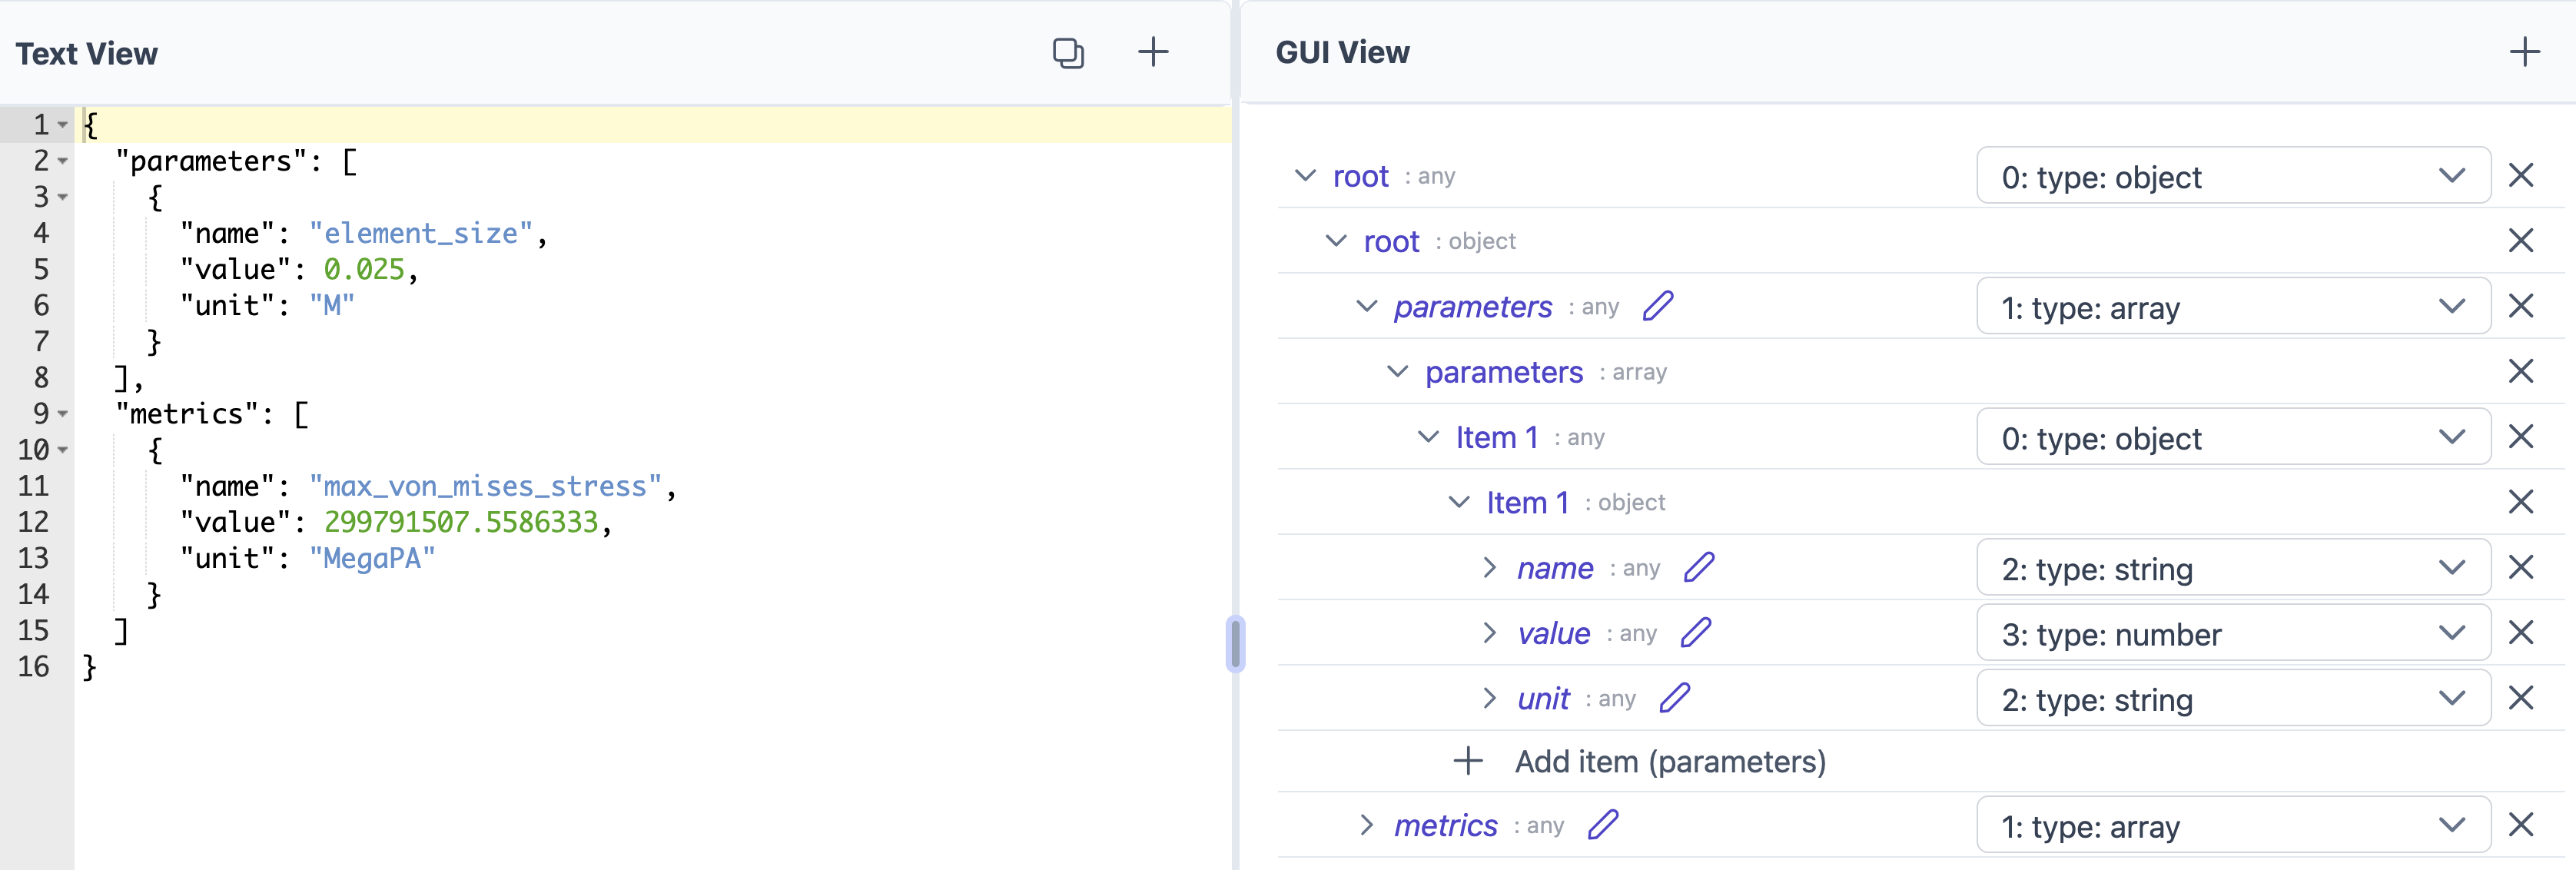
\includegraphics[width=.95\linewidth]{../figures/MC-JSON.png}
  \caption{A snapshot of MetaConfigurator's data editing interface, showing the JSON instance from Listing~\ref{lst:background_json_example}}
    \label{fig:metaconfigurator_interface:data}
\end{figure}


\begin{figure}[htbp]
  \centering
  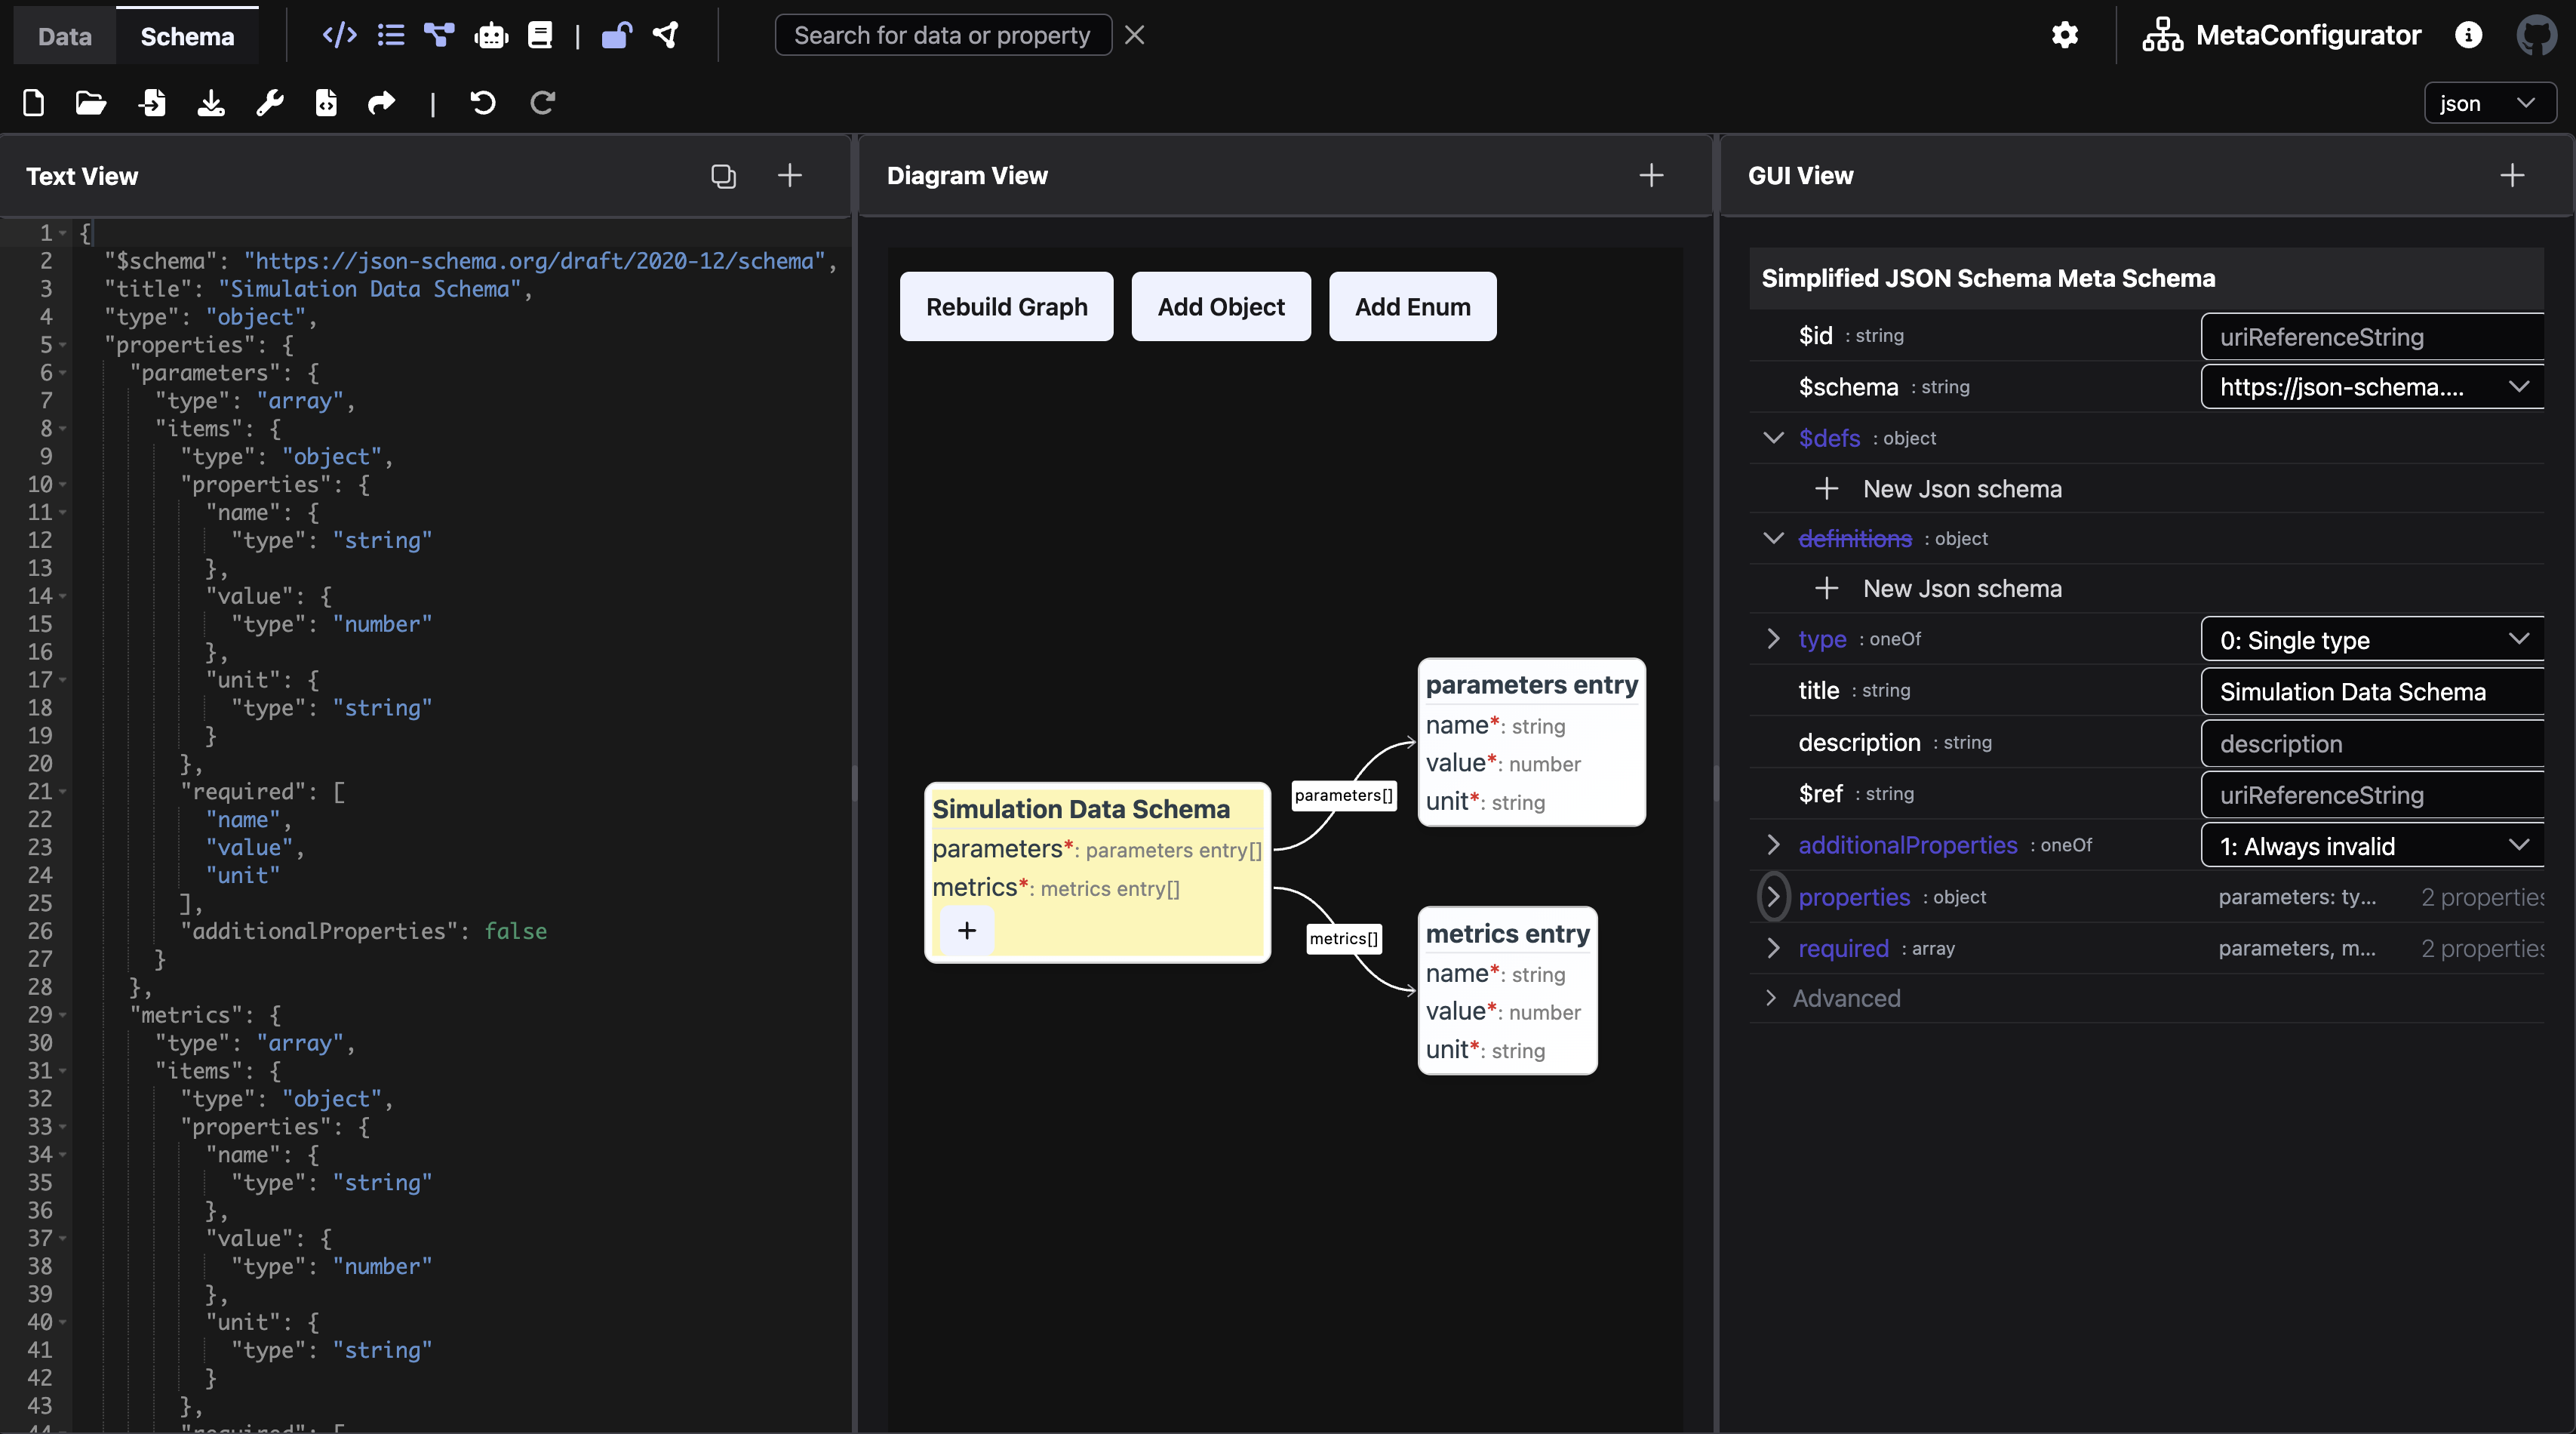
\includegraphics[width=.85\linewidth]{../figures/MC-JSON-Schema.png}
  \caption{A snapshot of MetaConfigurator's schema editing interface, showing the JSON Schema from Listing~\ref{lst:background_json_schema}}
  \label{fig:metaconfigurator_interface:schema}
\end{figure}


This combination of views gives users a continuous workflow from low-level text editing to guided schema-driven interaction, and reduces the effort needed to model, validate, and maintain structured data across different domains \cite{metaconfigurator2024,metaconfigurator2025datamodels}.

\newpage

\subsection{AI-Assisted Schema Engineering and Mapping}
\label{sec:background:metaconfigurator_ai}

Recent work extends MetaConfigurator with \gls{ai}-assisted support for schema creation, modification, and mapping from natural-language user input \cite{ai_assisted_schema_mapping_2025}. The approach combines \gls{llm}s with deterministic safeguards to improve reliability and usability.

In this workflow, the chat-like dialog is used for data-mapping tasks. Schema edits, in contrast, are applied directly in the schema editor rather than through a separate dialog; users can immediately inspect the result and revert undesired changes with the built-in Undo action. This keeps schema authoring interactive while preserving user control over incremental modifications.

For data transformation, the system generates mapping expressions from user input and executes these mappings deterministically. In the presented implementation, JSONata expressions are generated from an input document and a target schema, then validated and executed in a controlled pipeline. This separates \gls{ai}-based generation from rule execution and supports scalable transformation workflows across heterogeneous source formats.

\newpage

\subsection{Limitations for Semantic Web Integration}
\label{sec:background:metaconfigurator_limitations}

Despite its strong support for schema-driven data modeling, MetaConfigurator currently provides only limited support for Semantic Web technologies: while the platform enables the creation and validation of structured data using \gls{json} and JSON Schema, it has limited support for Linked Data representations. Currently, MetaConfigurator treats \gls{json} documents primarily as structured configuration data and does not interpret or expose their underlying \gls{rdf} semantics.

Several limitations arise from this restriction:

\begin{enumerate}
    \item \textbf{Lack of JSON-LD context authoring:}  
    Users cannot directly author or edit \gls{jsonld} contexts (e.g., the \texttt{@context} section that maps \gls{json} keys to ontology \glspl{iri}) in the data editing view. Although JSON-LD support allows defining context information in the schema editor, this functionality remains limited and is not available where instance-level data is authored, so linking data elements to ontologies still often requires manual editing outside the core data workflow.

    \item \textbf{No direct inspection or editing of RDF triples:}  
    MetaConfigurator does not provide mechanisms for inspecting or manipulating \gls{rdf} triples derived from the underlying \gls{json} data. As a result, users cannot directly view the semantic graph structure implied by \gls{jsonld} documents.

    \item \textbf{Lack of transformation from JSON to RDF:}  
    The platform lacks built-in mechanisms for transforming conventional \gls{json} documents into semantic representations. As discussed in Section~\ref{sec:background:rml}, technologies such as \gls{rml} enable declarative transformations from \gls{json} to \gls{rdf}, but such transformations are not currently integrated into MetaConfigurator's workflow.

    \item \textbf{Lack of semantic querying capabilities:}  
    MetaConfigurator does not support semantic querying of \gls{rdf} data. As described in Section~\ref{sec:background:sparql}, \gls{sparql} provides a standard mechanism for querying \gls{rdf} graphs and retrieving structured information from \glspl{kg}.

    \item \textbf{No visualization of RDF \glsentryshort{kg}s:}  
    \Glspl{kg} are often easier to understand when represented visually as nodes and relationships. However, the current platform does not provide mechanisms to visually explore \gls{rdf} triples or inspect the structure of the resulting \gls{kg}.
\end{enumerate}

To address these limitations, this thesis extends MetaConfigurator with an \textbf{RDF Authoring Panel} that integrates Semantic Web technologies directly into the schema-driven editing environment. 

\newpage

The main contributions of this thesis include:

\begin{enumerate}
    \item \textbf{Integration of RML Mapping Functionality into MetaConfigurator:}  
    The system integrates \gls{rml}-based mapping functionality into MetaConfigurator to transform conventional \gls{json} documents into \gls{jsonld}. This allows structured \gls{json} data created within the platform to be converted into \gls{rdf} triples that can be integrated into Semantic Web infrastructures.

    \item \textbf{RDF authoring and editing support:}  
    The RDF Authoring Panel allows users to directly inspect and edit \gls{rdf} data. This includes editing the \gls{jsonld} \texttt{@context} as well as creating and modifying \gls{rdf} triples within the interface.

    \item \textbf{Ontology-aware IRI auto-completion:}  
    The system integrates ontology lookup services that provide auto-completion for \glspl{iri} when authoring \gls{rdf} triples. This facilitates the reuse of existing ontologies and promotes semantic interoperability.

    \item \textbf{SPARQL querying support:}  
    The extension introduces the ability to query \gls{rdf} data using \gls{sparql}. This allows users to retrieve and analyze information from the generated \gls{kg} directly within the MetaConfigurator environment.

    \item \textbf{Interactive \glsentryshort{kg} visualization:}  
    The \gls{rdf} triples generated from \gls{jsonld} can be visualized as an interactive graph representation. This visualization enables users to explore entities and relationships within the \gls{kg} and understand the semantic structure of the data more easily.

    \item \textbf{AI-assisted SPARQL and RML authoring from user hints:}  
    Building on MetaConfigurator's existing \gls{ai}-assisted schema capabilities, this thesis introduces \gls{ai}-assisted generation of \gls{sparql} queries and \gls{rml} mappings from user-provided hints. Users can describe their intent in natural language and receive draft \gls{sparql} queries and \gls{rml} mapping definitions that can be reviewed and refined in the RDF Authoring Panel.
\end{enumerate}

By integrating these capabilities into MetaConfigurator, the platform evolves from a schema-based configuration editor into a tool that supports the full workflow of creating, transforming, querying, and exploring semantically enriched data.

\section{Related Work}
\label{sec:background:related_work}

Related work in this area spans several mature but often separate tool families: ontology engineering platforms, transformation tools that convert source data into \gls{rdf}, schema/metadata modeling environments for structured data, and libraries or engines for querying and validation. These families provide strong support for individual tasks, but integrated workflows that combine guided \gls{json} authoring, semantic transformation, \gls{rdf} curation, querying, and \gls{ai}-assisted support in a single user-facing environment are still uncommon.

\subsection{Ontology Engineering and \glsentryshort{kg} Platforms}

Protégé and WebProtégé are widely used for ontology engineering and collaborative ontology curation \cite{protege,webprotege}. Their strength is formal ontology modeling, but this also implies a relatively high entry barrier: users need to understand \gls{rdf}/\gls{owl} concepts and \glspl{iri}s before they can work productively \cite{janowicz2015geospatial,hogan2021knowledgegraphs}. In many practical settings, however, data already exists in traditional non-linked formats such as \gls{json}, \gls{xml}, \gls{csv}, or \gls{yaml}, and teams do not start from native \gls{rdf}. MetaConfigurator addresses this gap by supporting import and schema-driven editing of such existing formats \cite{metaconfigurator2024,metaconfigurator2025datamodels}; the RDF Authoring Panel could provide the next step as a bridge from conventional structured data to semantic data engineering.

Apache Jena provides a mature programmatic stack for \gls{rdf} processing, reasoning, and \gls{sparql} querying \cite{apache_jena}. GraphDB focuses on \gls{rdf} storage and query execution in production-oriented \gls{kg} settings \cite{graphdb}. These systems are strong back-end components, but typically require separate front-end layers for guided data entry and authoring workflows.

\subsection{Schema and Metadata Modeling for Structured Data}

LinkML is a schema-centric tool in this context. It follows a model-driven approach in which a single high-level schema can be used to generate multiple artifacts, including validation schemas and semantic representations such as \gls{jsonld} and \gls{owl} \cite{linkml}. This is highly valuable for maintaining consistency across data models and downstream implementations. At the same time, effective use of LinkML still requires substantial conceptual understanding of schema design, semantic modeling decisions, and artifact generation workflows, which can be challenging for domain users without prior Semantic Web experience. In addition, LinkML introduces yet another schema-language standard that users must learn alongside existing standards such as JSON Schema and \gls{rdf}, which can increase adoption overhead in practice.

The \gls{cedar} Workbench also improves metadata quality through ontology-assisted authoring in scientific contexts \cite{cedar_workbench}. However, as with other advanced modeling environments, the practical starting point in many projects is not a clean semantic model, but existing non-linked datasets in operational formats such as \gls{json}, \gls{xml}, \gls{csv}, or \gls{yaml}. For these scenarios, a bridge approach is needed: first support users in editing and structuring their existing data, then map it into \gls{rdf}. This is why declarative mapping approaches such as \gls{rml} are particularly suitable in our setting (Section~\ref{sec:background:rml}), and why MetaConfigurator is positioned as a gradual path from conventional structured data toward semantic \glsentryshort{kg} workflows rather than assuming that users begin directly with native \gls{rdf}.

\subsection{Transformation from Source Data to RDF}

Karma, OpenRefine (with \gls{rdf} extensions), and SPARQL-Generate support transformation from heterogeneous sources to \gls{rdf} \cite{karma,openrefine,sparql_generate}. These tools are strong choices when the main goal is mapping source records into triples. However, they are typically centered on the transformation step itself. In contrast, our approach targets a broader user workflow: preparing existing non-linked data, transforming it to \gls{rdf}, and then continuing with semantic authoring, inspection, and querying in one environment.

\subsection{Querying, Validation, and Programmatic RDF Processing}

\gls{rdf} validation and querying standards such as \gls{shacl} and \gls{sparql} are well established \cite{shacl_standard,sparql_standard}. For lightweight experimentation, \gls{jsonld} Playground provides quick inspection of contexts and \gls{rdf} output \cite{jsonld_playground}. RDFLib and Redland provide low-level programmatic \gls{rdf} processing \cite{rdflib,redland}. These tools are important ecosystem building blocks but are not, by themselves, unified authoring environments.

\subsection{Comparison of Semantic Web Editing Tools}

Table~\ref{tab:related_tools_comparison} compares a subset of Semantic Web editing tools across capabilities, including \gls{rdf} authoring, ontology integration, source-to-\gls{rdf} transformation, \gls{rdf} storage/query, visualization, and \gls{ai} assistance.

\begin{table}
\centering
\caption{Comparison of tools supporting RDF authoring and Semantic Web integration}
\label{tab:related_tools_comparison}
\renewcommand{\arraystretch}{1.2}
\begin{tabular}{lcccccc}
\hline
\textbf{Tool / Framework} 
& \rotatebox{90}{RDF Authoring} 
& \rotatebox{90}{Ontology Integration} 
& \rotatebox{90}{Source-to-RDF Transform.} 
& \rotatebox{90}{RDF Storage / Query} 
& \rotatebox{90}{Visualization}
& \rotatebox{90}{AI Assistance} \\
\hline
Protégé & \dingcheck & \dingcheck & -- & -- & \dingcheck & -- \\
WebProtégé & \dingcheck & \dingcheck & -- & -- & Limited & -- \\
Apache Jena & \dingcheck & \dingcheck & Limited & \dingcheck & -- & -- \\
LinkML & -- & \dingcheck & Partial & -- & -- & -- \\
SemTK~\cite{semtk} & \dingcheck & \dingcheck & Partial & \dingcheck & \dingcheck & -- \\
OpenRefine (RDF) & Limited & -- & \dingcheck & -- & -- & -- \\
SPARQL-Generate & -- & -- & \dingcheck & -- & -- & -- \\
JSON-LD Playground & Limited & -- & Limited & -- & Limited & -- \\
RDFLib & \dingcheck & Limited & -- & Partial & -- & -- \\
Redland RDF & \dingcheck & Limited & -- & Partial & -- & -- \\
\hline
\end{tabular}
\end{table}

\begin{table}
\centering
\caption{Rating scale used in Table~\ref{tab:related_tools_comparison}}
\label{tab:rating_scale}
\renewcommand{\arraystretch}{1.2}
\begin{tabular}{l>{\raggedright\arraybackslash}p{10cm}}
\hline
\textbf{Symbol / Term} & \textbf{Meaning} \\
\hline
\dingcheck & Native, first-class support \\
\cdashline{1-2}
Partial & Substantial but scope-limited support (often programmatic rather than end-user-focused) \\
\cdashline{1-2}
Limited & Basic or indirect support (e.g., plugin-based, narrow subset, or lightweight/read-only capability) \\
\cdashline{1-2}
-- & Not a core capability \\
\hline
\end{tabular}
\end{table}


\newpage

\section{Research Gap and Positioning of This Thesis}

Although these tools provide strong support for individual Semantic Web tasks, several limitations remain for practical data workflows:

\begin{itemize}
    \item \textbf{Fragmented workflows:} Modeling, mapping, querying, and visualization are often distributed across multiple tools, requiring users to switch between different environments to complete a single data integration task \cite{hogan2021knowledgegraphs}.

    \item \textbf{High technical entry barrier:} Effective use often requires advanced knowledge of \gls{owl}, \gls{rdf}, \gls{sparql}, and mapping languages, which limits accessibility for domain scientists who are not Semantic Web experts \cite{janowicz2015geospatial}.

    \item \textbf{Gap between structured JSON editing and RDF transformation:} In practice, much scientific data is authored and maintained in hierarchical formats such as \gls{json}. While standards such as \gls{jsonld} provide a bridge to linked data \cite{jsonld2014}, moving from conventional \gls{json} structures to \gls{rdf} still often requires separate mapping artifacts and additional tools (e.g., \gls{r2rml}/\gls{rml}) \cite{das2012r2rml,dimou2014rml}.

    \item \textbf{Limited end-to-end support in one user interface:} Most tools focus on a single task—such as ontology editing, mapping definition, or querying—rather than supporting the entire workflow from data authoring and transformation to validation, querying, and graph exploration in a unified environment.

    \item \textbf{Limited AI support in semantic authoring workflows:} Despite recent advances in generative \gls{ai}, assistance for generating artifacts such as \gls{sparql} queries or \gls{rml} mappings from natural-language descriptions of user intent is still rarely integrated into Semantic Web authoring tools.
\end{itemize}

This thesis addresses these gaps by extending MetaConfigurator from a schema-guided data modeling tool into an integrated \gls{rdf} authoring environment. In particular, it supports a continuous workflow from \gls{json} authoring to \gls{jsonld}/\gls{rdf} transformation, ontology-aware triple editing, integrated \gls{sparql} querying, graph visualization, and \gls{ai}-assisted drafting of \gls{sparql} queries and \gls{rml} mappings.
